\documentclass[a4paper]{article}

\usepackage[spanish]{babel}
\usepackage[utf8]{inputenc}
\usepackage[T1]{fontenc}
\usepackage{float}
\usepackage{graphicx}
\usepackage{amsmath,amssymb,amsfonts}
\usepackage{subcaption}
\usepackage[most]{tcolorbox}
\usepackage{xcolor}
\usepackage[a4paper,top=1cm,bottom=1.5cm,left=3cm,right=3cm,marginparwidth=2.5cm]{geometry}
\usepackage{pgfplots}
\usepackage{palatino}
\pgfplotsset{compat=1.18}
\usetikzlibrary{decorations.pathreplacing,babel}

\newif\ifprintanswers
\printanswerstrue

\definecolor{miazul}{RGB}{25,43,191}

% Definición de solution con recuadro
\NewEnviron{solution}{%
  \ifprintanswers
    \begin{tcolorbox}[
      colframe=black,     % color del borde
      colback=white,      % fondo blanco
      boxrule=0.8pt,      % grosor de la línea
      arc=0pt,            % esquinas agudas
      left=4pt,           % espacio interior izquierdo
      right=4pt,          % espacio interior derecho
      top=4pt,            % espacio interior superior
      bottom=4pt,         % espacio interior inferior
      before skip=0.5\baselineskip,
      after skip=0.5\baselineskip
    ]
      \textbf{\textit{Respuesta:}}\quad
      \BODY
      \hfill\(\triangleright\)
    \end{tcolorbox}
  \fi
}

\begin{document}

\noindent\makebox[\textwidth]{%
  \texttt{joamartine@fen.uchile.cl}%
  \hfill%
  Magíster en Análisis Económico
}

\vspace{5mm}

\begin{center}
  {\large \textbf{Finanzas Internacionales, Otoño 2026}}\\[4pt]
  {\large \textbf{Ayudantía 3}}
\end{center}

\vspace{3mm}

\section*{Comentes}

\begin{enumerate}
    \item[a)] Explique según el modelo HBS cómo un aumento de la productividad de los bienes transables de un país se traduce en una apreciación del tipo de cambio real. También explique por qué un aumento de productividad de los no transables deprecia el tipo de cambio real.

    \begin{solution}

        \textbf{Un aumento en la productividad del sector de bienes transables aprecia el tipo de cambio real.} El modelo HBS considera que un país abierto al comercio tiene dos sectores, bienes transables ($T$) y bienes no transables ($N$). Si bien hay movilidad de trabajadores entre estos sectores, cada uno tiene una productividad exógena $a_T$ y $a_N$. Hay dos puntos a considerar en este contexto:
        \begin{itemize}
            \item Ley del precio único $$P_T = e\cdot P_T^*.$$
            \item Los salarios en ambos sectores son iguales $$W = P_T\cdot a_T.$$
        \end{itemize}
        Luego, si por algún shock exógeno $a_T$ aumenta y $P_T$ se mantiene (constante por ley de precio único), entonces se deben ajustar los salarios al alza. El aumento salarial aumenta el precio de los no transables mientras que $a_N$ se mantiene constante, $$\uparrow W = \uparrow P_N\cdot a_N.$$ Finalmente, esto impulsa al alza el nivel general de precios, $$\downarrow q = \frac{eP^*}{\uparrow P}.$$

        \textbf{Un aumento de productividad en el sector de bienes no transables genera una depreciación del tipo de cambio real.} Un aumento en la productividad de los bienes no transables presiona al alza el salario; como el salario se determina también por la productividad y nivel de precios de los transables y estos están dados, los salarios se mantienen, y el ajuste finalmente se da por un abaratamiento de los bienes no transables, $$P_T\cdot a_T = W = \downarrow P_N \cdot \uparrow a_N.$$ Esto reduce el nivel de precios del país y por lo tanto deprecia el tipo de cambio real, $$\uparrow q = \frac{eP^*}{\downarrow P}.$$
    \end{solution}

    \item[b)] Un aumento en el gasto de gobierno que se orienta principalmente a bienes no transables puede generar una apreciación del tipo de cambio real, incluso si el tipo de cambio nominal se mantiene constante.

    \begin{solution}
        Verdadero. El mayor gasto público en bienes no transables incrementa su demanda. Como estos bienes no se comercian internacionalmente y su oferta es rígida en el corto plazo, sus precios aumentan (\( P_N \uparrow \)). Esto eleva el nivel general de precios internos (\( P \)), lo que implica una apreciación del tipo de cambio real:
        \[
        q = \frac{e \cdot P^*}{P} \downarrow
        \]
        Este efecto se produce incluso si el tipo de cambio nominal (\( e \)) permanece constante, ya que la apreciación real proviene del aumento de precios internos y no de una variación en el tipo de cambio nominal.
    \end{solution}

    \item[c)] El tipo de cambio real de Chile ha evolucionado de la siguiente forma:
    \begin{center}
        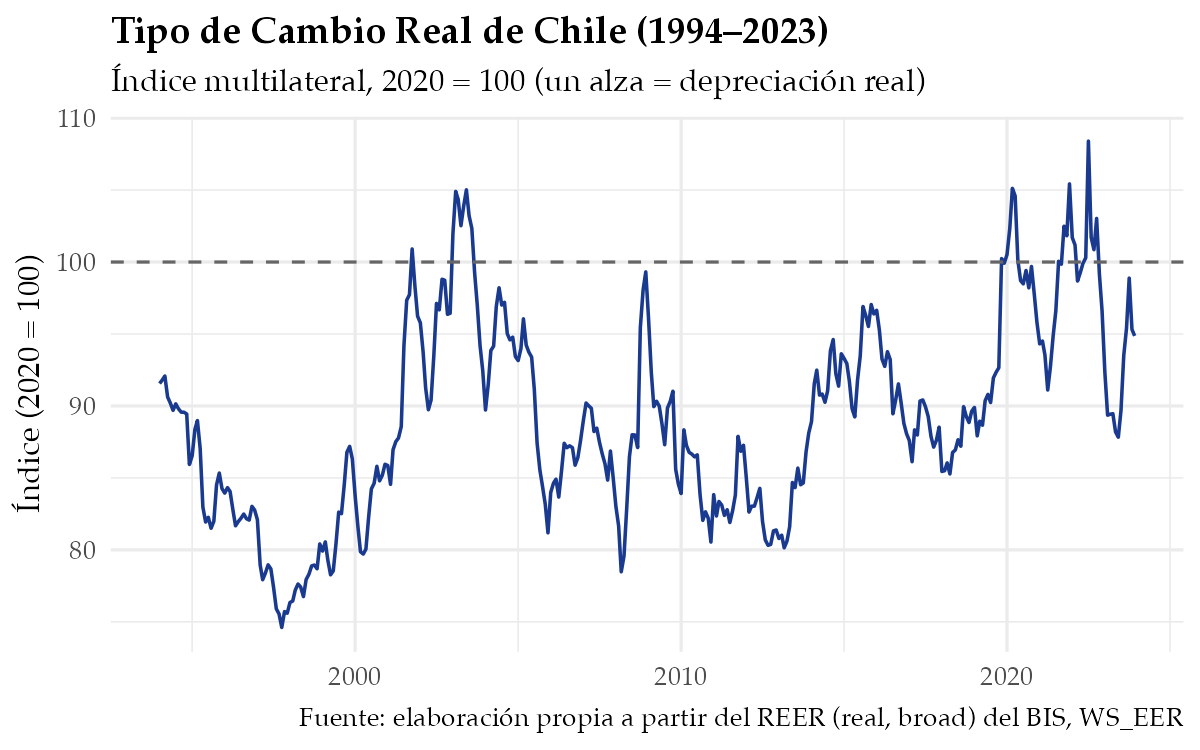
\includegraphics[width=10cm]{tcr_rcode/outputs/tcr_chile.png}
    \end{center}
    Explique qué factores (fundamentales y asociados al ciclo) pueden explicar la evolución del tipo de cambio real en los siguientes períodos: 1990--1997; 1998--2003; 2003--mediados de 2008; y el periodo 2020--2021. Utilice un factor para cada período. En particular, discuta a través de qué mecanismo el factor elegido por usted explica la evolución del tipo de cambio real en el período de análisis (cuatro periodos de análisis; cuatro factores distintos).

    \begin{solution}
        Recuerde la convención del gráfico: un alza del índice es una \emph{depreciación} real ($q\uparrow$) y una caída es una \emph{apreciación} ($q\downarrow$). Asignamos un factor distinto a cada período:
        \begin{itemize}
            \item \textbf{1990--1997 (apreciación): diferenciales de productividad (Balassa-Samuelson).} Un aumento en la productividad de los transables en Chile respecto del resto del mundo eleva los salarios de toda la economía (incluyendo los no transables). Ese mayor salario sube el precio de los no transables y genera una apreciación real.
            \item \textbf{1998--2003 (depreciación): riesgo país / diferencial de tasas.} La crisis asiática y rusa gatilla un \emph{sudden stop}: aumenta el riesgo país, suben los diferenciales de tasas exigidos, salen capitales y el tipo de cambio real se deprecia en el corto plazo.
            \item \textbf{2003--mediados de 2008 (apreciación): términos de intercambio.} El boom del cobre eleva el precio de lo que Chile exporta respecto de lo que importa. El mayor precio de los transables sube los salarios locales y los precios internos en relación con los externos, apreciando el TCR.
            \item \textbf{2020--2021 (depreciación): caída en los activos externos netos.} Los retiros de fondos de pensiones obligan a las AFP a liquidar activos en el exterior; la caída en la posición de activos externos netos (junto con la mayor incertidumbre) presiona el tipo de cambio nominal al alza y deprecia el TCR.
        \end{itemize}

        Otros potenciales factores:
        \begin{itemize}
            \item \textbf{Gasto de gobierno.} Si el gasto es más intensivo en bienes no transables, un aumento de éste tiende a apreciar el TCR y una caída tiende a depreciarlo.
            \item \textbf{Menor crecimiento futuro.} Reduce la demanda hoy, lo que baja los precios internos y deprecia el TCR.
            \item \textbf{Aumento en deuda externa neta} que requiere mayores superávits comerciales y, por lo tanto, un TCR más depreciado.
        \end{itemize}
    \end{solution}

    \item[d)] La administración de Estados Unidos anunció un eventual arancel del 50\% sobre el cobre. ¿Cómo afectaría a los términos de intercambio y tipo de cambio real de Chile?

    \begin{solution}
        \textbf{Si Estados Unidos tiene poder de mercado:} el arancel disminuye el precio mundial del cobre y empeora los términos de intercambio. Menores precios del sector de transables disminuyen los salarios y los precios de los no transables también se ajustan a la baja, causando una depreciación real del tipo de cambio.

        \textbf{Si Estados Unidos no tiene poder de mercado:} el arancel solo aumenta el precio de importación en Estados Unidos dada su baja elasticidad precio de la demanda; por lo tanto el precio mundial se mantiene y no hay cambios en los términos de intercambio.
        \vspace{3mm}

        \textit{Nota:} Apenas anunciado, el precio del cobre subió. Esto se explicaría principalmente por compras spot del metal ante un aumento en el precio esperado en Estados Unidos (acumulación de inventarios).
    \end{solution}

    \item[e)] Controlar el déficit en cuenta corriente en el primer período mediante un alza de la tasa de interés puede tener efectos apreciatorios sobre el tipo de cambio real.

    \begin{solution}
        \textbf{Falso}, el efecto va en sentido contrario en este modelo. Controlar el déficit significa reducirlo, es decir, llevar la cuenta corriente hacia el equilibrio (menos negativa). Un alza de la tasa de interés reduce la inversión y, con ahorro dado, achica la brecha $I-S$ y por tanto el déficit. Pero para que el saldo comercial mejore (un menor déficit exige un $NX$ mayor) el tipo de cambio real debe \emph{depreciarse}: con $X(q)$ creciente y $M(q)$ decreciente, un $NX$ mayor requiere $q\uparrow$. Por lo tanto controlar el déficit \textbf{deprecia} el TCR en el primer período, no lo aprecia. Es exactamente lo que se obtiene en el ejercicio del Matemático, donde el control lleva $q_1$ de $0{,}983$ a $1{,}033$.

        El canal financiero de ``defensa con tasas'' (una tasa alta atrae capitales y aprecia) no aplica aquí, porque mayores entradas de capital \emph{agrandarían} el déficit, contradiciendo el objetivo de controlarlo.
    \end{solution}

    \item[f)] Si una economía presenta un alto riesgo soberano, enfrentará una tasa de interés externa más alta, lo que tiende a reducir su inversión, mejorar su cuenta corriente y depreciar su tipo de cambio real.

    \begin{solution}
        \textbf{Verdadero.} Una economía con riesgo soberano enfrenta una \textit{prima de riesgo} sobre la tasa de interés internacional, por lo que su tasa efectiva es
        \[
        r = r^* + \text{prima}.
        \]
        Un mayor \( r \) reduce la inversión. Si el ahorro nacional se mantiene constante, la brecha $I-S$ cae y la cuenta corriente mejora (menor déficit o mayor superávit).

        En cuanto al tipo de cambio real, ambos canales apuntan a una \emph{depreciación}:
        \begin{itemize}
            \item Una cuenta corriente que mejora exige un $NX$ mayor, lo que en este modelo requiere una depreciación real (\( q \uparrow \)).
            \item El mayor riesgo gatilla salida de capitales, presiona al alza el tipo de cambio nominal (\( e \uparrow \)) y, si los precios internos no se ajustan tan rápido, deprecia el tipo de cambio real (\( q \uparrow \)).
        \end{itemize}
        Por tanto, el riesgo soberano mejora la cuenta corriente mediante la contracción de la inversión y deprecia el tipo de cambio real, tal como afirma el enunciado.
    \end{solution}

\end{enumerate}

\section*{La cuenta corriente y el tipo de cambio intertemporal}

Considere una economía que existe por dos períodos: tiene un PIB de 100 y un nivel de ahorro nacional de 24 (en una unidad cualquiera, pero todas las otras magnitudes reales se expresan en la misma unidad), y es insensible a las tasas de interés. La inversión está dada por: $$I = 42 - 2r.$$

Donde $r$ mide la tasa de interés real medida en porcentaje. La economía es abierta a los flujos financieros internacionales y la tasa de interés a la cual el mundo está dispuesto a prestarle y pedirle prestado a esta economía es de 4\% ($r = 4$) por año.

Las exportaciones e importaciones están dadas por:
\begin{align*}
X &= 60q - 20 \\
M &= 108 - 60q
\end{align*}
Donde $q$ es el tipo de cambio real.

El hecho de que esta economía viva por dos períodos significa que solo ahorra e invierte en el período 1 (note bien que el ahorro total en el período 2 es 0), y en el período 2 cancela sus compromisos con el exterior (y vive de lo que le queda). Al principio no hay deuda externa.

\begin{enumerate}
  \item[a)] Calcule el tipo de cambio real de equilibrio en ambos períodos. ¿Cuál es la intuición detrás de su resultado?
  \begin{solution}
      \textbf{Primer período:} Para el primer período, con $r = 4$,
      \begin{align*}
          I = S_N + S_E &= 42 - 2r \\
          24 + S_E &= 34 \\
          S_E &= 10.
      \end{align*}
      Sabemos que el ahorro externo es el déficit de cuenta corriente; consideramos que no hay pagos ni ingresos por factores con el exterior ($F = 0$), por lo tanto, por cómo se comportan importaciones y exportaciones, podemos escribir $$S_E = -CC = M + rF - X \implies 10 = 108 - 60q - 60q + 20.$$ Despejando, $q_1 = 0{,}983$.

      \textbf{Segundo período:} El saldo de cuenta corriente es $-10$; tenemos déficit, por lo que pagamos intereses a una tasa $r = 4$. La igualdad que se cumple es que la cuenta corriente más intereses tiene que ser igual a la balanza comercial (recordemos $F = 0$):
      \[
      CC_1(1+r) = X - M \implies -10(1+0{,}04) = 108 - 60q - 60q + 20 \implies -10{,}4 = 128 - 120q,
      \]
      de donde $q_2 = 1{,}153$.

      \textbf{Intuición:} la economía parte sin deuda. En el período 1 invierte más de lo que ahorra (déficit de cuenta corriente, entrada de capitales), lo que va de la mano de un TCR relativamente apreciado ($q_1 = 0{,}983$). En el período 2 debe generar un superávit comercial para pagar la deuda con intereses, lo que requiere un TCR depreciado ($q_2 = 1{,}153$). El tipo de cambio real se deprecia entre períodos para revertir el saldo comercial.
  \end{solution}

  \item[b)] Suponga ahora que las autoridades económicas deciden que esta economía no puede tener un déficit en la cuenta corriente mayor de 4 del PIB durante el primer período. Calcule la tasa de interés de equilibrio en el período 1 y el tipo de cambio real de equilibrio en ambos períodos.
  \begin{solution}
      Dado $S_E = 4$ e $I = 28$, del equilibrio de oferta y demanda $$28 = 24 + 4 = 42 - 2r \implies r = 7.$$ Seguimos el mismo procedimiento del ítem anterior para calcular el tipo de cambio real en ambos períodos:
      \begin{itemize}
          \item[1.] Primer período: $$4 = 108 - 60q - 60q + 20 \implies q_1 = 1{,}033.$$
          \item[2.] Segundo período (con intereses): $$-4(1+0{,}07) = 108 - 60q - 60q + 20 \implies q_2 = 1{,}102.$$
      \end{itemize}
  \end{solution}

  \item[c)] Comente las consecuencias sobre el tipo de cambio real de tener una política de controlar el déficit en la cuenta corriente, en particular sobre el nivel y la estabilidad en el tiempo del tipo de cambio real.
  \begin{solution}
      El control del déficit deprecia la moneda en el primer período, pues entran menos capitales, con lo cual aumenta el precio de la moneda extranjera ($q_1$ pasa de $0{,}983$ a $1{,}033$).

      En el segundo período el tipo de cambio es más apreciado que en la situación sin control ($q_2$ pasa de $1{,}153$ a $1{,}102$): como el déficit es menor, se paga una menor deuda.

      En consecuencia, el tipo de cambio real tiene una trayectoria más estable cuando se aplica el control: varía entre $1{,}033$ y $1{,}102$ con control, frente a $0{,}983$ y $1{,}153$ sin control.
  \end{solution}
\end{enumerate}

\end{document}
